\documentclass[tikz,border=5mm]{standalone}
\usepackage{tikz}
\usetikzlibrary{arrows.meta, positioning, shapes.geometric, calc, backgrounds, fit, matrix, patterns, decorations.pathmorphing, shadows}

% --- COLOR DEFINITIONS ---
\definecolor{Garnet}{HTML}{73000A}
\definecolor{CSecondaryRed}{HTML}{CC2E40}
\definecolor{CBlue}{HTML}{466A9F}
\definecolor{CDark}{HTML}{1F414D}
\definecolor{COlive}{HTML}{65780B}
\definecolor{CLime}{HTML}{CED318}
\definecolor{CGold}{HTML}{A49137}
\definecolor{CGrayLight}{HTML}{E5E5E5}
\definecolor{CGrayDark}{HTML}{555555}
\definecolor{CWhite}{HTML}{FFFFFF}
\definecolor{CBlack}{HTML}{000000}

\begin{document}

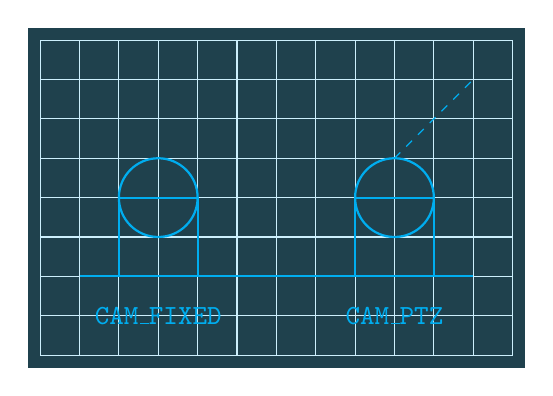
\begin{tikzpicture}[background rectangle/.style={fill=CDark}, show background rectangle]
    \draw[help lines, step=0.5, cyan!20, thin] (-3,-1) grid (3,3);
    
    % Cam 1
    \draw[cyan, thick] (-2, 0) rectangle (-1, 1);
    \draw[cyan, thick] (-1.5, 1) circle (0.5);
    \node[cyan, font=\ttfamily] at (-1.5, -0.5) {CAM\_FIXED};
    
    % Cam 2
    \draw[cyan, thick] (1, 0) rectangle (2, 1);
    \draw[cyan, thick] (1.5, 1) circle (0.5);
    \draw[cyan, dashed] (1.5, 1.5) -- (2.5, 2.5); % Axis
    \node[cyan, font=\ttfamily] at (1.5, -0.5) {CAM\_PTZ};
    
    \draw[cyan, thick] (-2.5, 0) -- (2.5, 0);
\end{tikzpicture}

\end{document}
